\documentclass[blue]{LRSguildcamp1}
\begin{document}
\name{\bWorld{}}
You live in a world of superhumans.  Many of these superhumans -- almost all of them -- identify as either a hero, someone who protects civilians and property and respects the law, or a villain, someone who often sees cities as territory to be taken and controlled, and the civilians in it as useful laborers or, often, potential sources of income.  In the past, heroes and villains often worked alone, but over time nationwide alliances of heroes and villains developed: the \cHeroLeague{\intro}, and the \cVillainCompact{\intro}.  Members of the \cHeroLeague{\intro} often receive government support and are indemnified against the cost of property damage caused during fights with villains.  Members of the \cVillainCompact{\intro} agree to a truce amongst each other, help each other escape prison, and share a national database of skilled minions for hire.

Though heroes are generally viewed as upstanding defenders of the innocent, many villains are seen as independent, audacious, charming, and savvy.  Many civilians might not even mind living under a villain with a light touch -- is a little protection money really different from one more tax?

The presence of superpowers often runs in families, though even related superhumans usually exhibit completely unrelated powers.  It is not unknown, however, for unpowered humans' children to develop superpowers.

Even superhumans have lives and families, however, and sometimes need to take time off.  Generally, they will hire city-sitters -- minions, extra security forces, or more often, younger or D-list superhumans who can at least take care of simple tasks.  City-sitting is highly valued in the resum\'e of a young hero or villain, and is often expected of young superhumans before they take responsibility for a territory of their own.

Everybody has to go to high school and young super teens are no exception. \pSuperSchool{} is a four year boarding school that serves a 1400 member student body. Students must pass a curriculum that is compliant with the Department of Education Guidelines and receive a degree that is accepted at all accredited universities. Students with super abilities are taught how to handle and control them safely. They can receive a certification to use their power outside of school during their lives. Students also have electives including learning to apply their abilities to trades and industrious uses.  If students join the \cHeroLeague{\intro}, they received special training in how to use their powers to help the police keep the peace and gain access to internships with various heroes. 

The public often finds superhumans fascinating, and often considers them celebrities in their own right, with the \cHeroLeague{\intro} and \cVillainCompact{\intro} often in competition for public opinion.  The Internet abounds with rumors, news, fact and (fan)fiction.  The most popular rumor site about superhumans on the Internet is \pTweenwebsite{}. \pTweenwebsite{} is a one-stop website for all things super. The public loves their celebrities, and super hero and super villains are the cream of the crop. The site is a massive aggregation of fan theories and burning questions.  Users who've dug up the answers to fan theories and questions about various superhumans gain levels of InTheKnow, which grants them increased access, prestige, and expanded audiences for their posts. The levels are \textit{A bit InTheKnow}, \textit{Well InTheKnow}, \textit{Solidily InTheKnow}, and \textit{Epically InTheKnow}.

Today at 3pm, members of the legendary Kaper family fo superhumans are gathering for a family reunion organized by the family \cGrandma{\familyleader}, \cGrandma{\intro}.  \cGrandma{\Theyhave} scheduled a sit-down dinner in the dining room for 5:30pm.  As most of the family have cities to defend, however, everyone will need to leave promptly at 6.

Here is a list of superhumans in or associated with the legendary Kaper family:

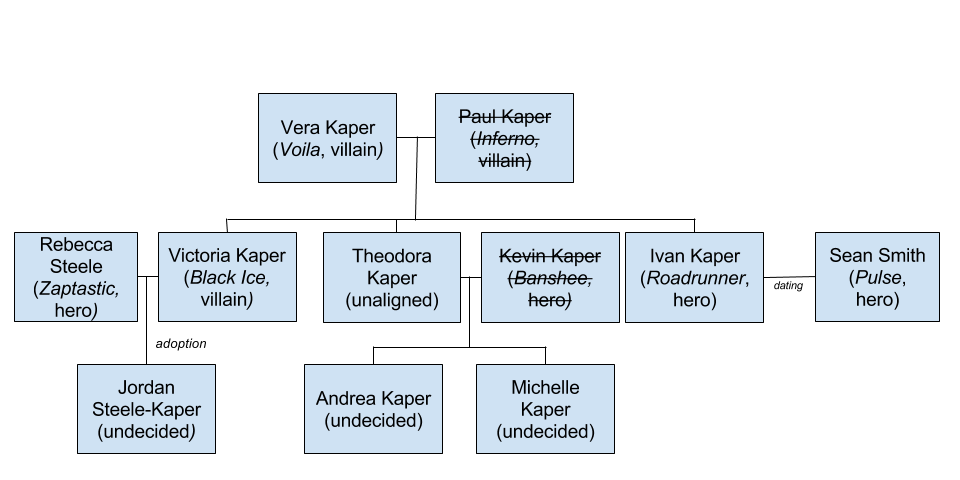
\includegraphics[width=0.8\textwidth]{Familytree.png}
\\
\begin{tabular}{l|l|l|p{0.35\linewidth}|p{0.1\linewidth}|p{0.1\linewidth}}
{\bf Name} & {\bf Pronoun} & {\bf Super name} & {\bf Reputation} & {\bf Allegiance} & {\bf Power} \\ \hline
\cGrandma{\intro} & \cGrandma{\they} & \cGrandma{\MYsupername} & A legendary supervillain, thief and occasional celebrity abductor. & Independent \cGrandma{\villain} & 
\cGrandma{\MYsuperpower} \\ \hline
\cGS{\intro} & \cGS{\they} & \cGS{\MYsupername} & Famed supervillain and \cGS{\spouse} of \cGrandma{}.  & Deceased \cGS{\villain} & \cGS{\MYsuperpower} \\ \hline
\cOldest{\intro} & \cOldest{\they} & \cOldest{\MYsupername} & Supervillain of \pCityO{}. Attractive, audacious, and ruthless.  Oldest child of \cGrandma{\intro}. In a torrid affair with \cOS{}. & \cVillainCompact{\intro} & \cOldest{\MYsuperpower} \\ \hline
\cOS{\intro} & \cOS{\they} & \cOS{\MYsupername} &  Superhero of \pCityO{}.  Attractive, practical, and determined.  In a torrid affair with \cOldest{}. & \cHeroLeague{\intro} & \cOS{\MYsuperpower} \\ \hline
\cArchitect{\intro} & \cArchitect{\they} & \cArchitect{\MYsupername} & Famous architect based in \pCityArchitect{}; does not use their superpowers.  Middle child of \cGrandma{\intro}. & Unaligned & \cArchitect{\MYsuperpower} \\ \hline
\cAS{\intro} & \cAS{\they} & \cAS{\MYsupername} & Spouse of \cArchitect{\intro}, and \cAS{\parent} of \cTeen{} and \cTween{}.  & Deceased \cAS{\hero} & \cAS{\MYsuperpower} \\ \hline
\cYoungest{\intro} & \cYoungest{\they} & \cYoungest{\MYsupername} & Upstanding superhero of \pCityYoungest{}.  Youngest child of \cGrandma{}. & \cHeroLeague{\intro} & \cYoungest{\MYsuperpower} \\ \hline
% \cYS{\intro} & \cYS{\they} & & Relatively unknown superhero with an ambiguous past.  \cYS{\SO} of \cYoungest{\intro}. & Amplifies other superhumans' powers \\ \hline
\cGrad{\intro} & \cGrad{\they} & \cGrad{\MYsupername} & Only child of \cOldest{} and \cOS{}.  Just graduated super college. & Undecided & \cGrad{\MYsuperpower} \\ \hline
\cTeen{\intro} & \cTeen{\they} & \cTeen{\MYsupername} & Older child of \cArchitect{}.  Reportedly something of a hellion. & Undecided & \cTeen{\MYsuperpower} \\ \hline
\cTween{\intro} & \cTween{\they} & \cTween{\MYsupername} & Younger child of \cArchitect{}.  Known in the family as a conspiracy theorist.  Choosing a high school to go to. & Undecided & \cTween{\MYsuperpower} \\ \hline
\end{tabular}

\end{document}
